\NEW{
\section{\newname: \name with Dynamic Bandwidth Separation}
\label{sec:dynamic}

\begin{figure}[t]
  \centering
  %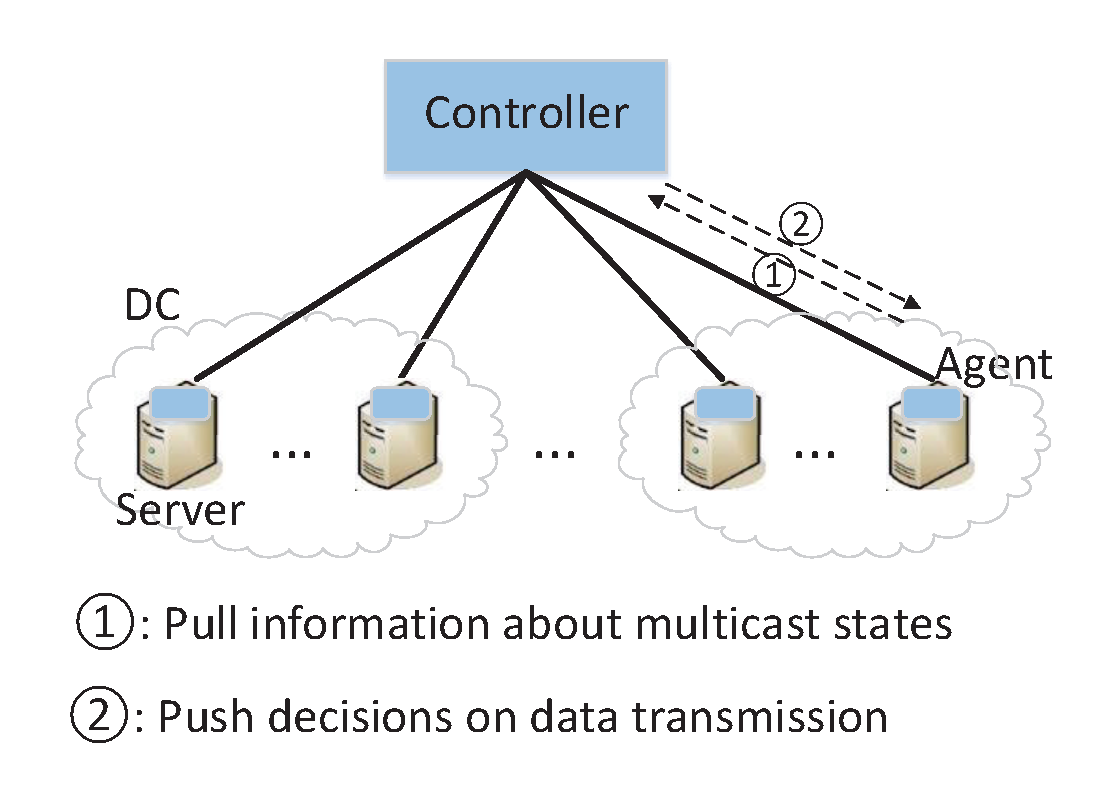
\includegraphics[width=2in]{images/framework.eps}
  \includegraphics[width=3.4in]{images/bds+.pdf}
    \vspace{-0.2cm}
  \tightcaption{\NEW{Logical diagram of \newname's dynamic bandwidth separation.}}
  \label{fig:bayes}
%\vspace{-0.4cm}
\end{figure}

\name performs well under fixed network separation, but in the mixed deployment situations where online traffic and offline traffic shares the same server I/O, it will results in low link utilizations when online traffic reduces: bulk data transfer will never occupy any bandwidth exceeds the safety threshold even though online traffic is far below the reserved bandwidth (see \Section\ref{subsec:motivation:baseline}).

So we further present an enhanced version of \name, called \newname, which achieves dynamic bandwidth separation with online traffic in a real-time manner, by continuously predicting online traffic changes and automatically adjusting the scheduling decisions, to fully utilize network bandwidth accordingly. To be specific, \newname automatically adjust the scheduling results under different network conditions: if online traffic encounters its peak, \newname shirks its occupied bandwidth to avoid congestions, while online traffic encounters its valley, \newname aggressively uses more bandwidth to make full use of the residual bandwidth.

To achieve this, \newname adopts a customized online traffic prdiction algorithm, which identifies the changes of server bandwidth usage, and triggers re-scheduling to adjust bandwidth allocation to the bulk-data transfer. Figure~\ref{fig:bayes} shows the logical diagram of \newname's dynamic bandwidth separation. The Network Change Monitor reads the agent observations (bandwidth usage) and executes \textit{K-Sigma} and a change point detection algorithm. \textit{K-Sigma} is responsible to predict the bandwidth by observing historical data. The change point detection is responsible for updating the changes based on agent observations and then it will adjust the historical data for \textit{K-Sigma} in order to make more accurate bandwidth prediction.

\subsection{Design Logic}
\label{subsec:dynamic:prediction}
%\mypara{Approaches to detect online traffic changes}
In order to detect online traffic changes and dynamically adjust configurations, the basic method is like exponentially weighted moving average (EWMA) control scheme, \textit{k-sigma} \cite{roberts1959control,lucas1990exponentially}, which calculates the mean and standard deviation of agent observations. Such approaches sometimes result in continual reconfigurations even when the network is (statistically) stationary (since samples may vary in time series). But it encounters a  challenge when predicting the available bandwidth: When we put more importance to the recent values as a reference (i.e., $k$ is small), there will be an obvious oscillation in the predicted value, which introduces unnecessary reschedules. When we put more importance to the historical values as references (i.e., $k$ is large), the predicted value will not be affected timely when a change point is suddenly detected, so that the system becomes insensitive to network changes.
%1) The other is the change point detection algorithm, which is the identifications of abrupt changes of sequential data. Such algorithms offers both online and offline processing methods, while offline methods \cite{smith1975bayesian,stephens1994bayesian,barry1993bayesian,green1995reversible} require the complete data in full time series to generate samples from the posterior distribution over change point locations, online methods \cite{page1955test,desobry2005online,lorden1971procedures} can generate an accurate distribution of the next unseen data with only already observed data. 

%\mypara{Change point detection algorithms}
To address the above problem, \newname combines \textit{k-sigma}  with  a change point detection algorithm \cite{adams2007bayesian}.  The change point detection algorithm, which is the identifications of abrupt changes of sequential data. Such algorithms offers both online and offline processing methods, while offline methods \cite{smith1975bayesian,stephens1994bayesian,barry1993bayesian,green1995reversible} require the complete data in full time series to generate samples from the posterior distribution over change point locations, online methods \cite{page1955test,desobry2005online,lorden1971procedures} can generate an accurate distribution of the next unseen data with only already observed data.  In \newname, we address this problem by adjusting the sliding $k$ of \textit{k-sigma}. Specifically, we set an upper bound $\textsc{K}$ for the EWMA algorithm, $k$ is set to be $\textsc{K}$ when there is no change points, and will be reset to $0$ once a change point is detected, and then gradually increase to $\textsc{K}$. We implemented our customized algorithm based on \cite{adams2007bayesian} (with code can be found in \cite{BOCDcode}) into the Network Change Monitor.

\subsection{Integrated to \name}
\subsubsection{Online traffic prediction algorithm}


%\mypara{Traffic Prediction}
During a scheduling cycle $\Delta T_k$ in \name, Network Change Monitor is continually fed with a series of agent observations of server throughput (bandwidth usage), which is used to predict the available bandwidth in the next scheduling cycle. To get the bandwidth usage, the Network Change Monitor periodically reads the record in process activity monitor on servers. For particular servers, they continuously log processing activities (including throughput) and send the sampled summed throughput to the Network Change Monitor. In this way, any network changes occurred during the bulk data downloading can be timely detected.

%chooses a change point detection algorithm to predict online traffic for two reasons. First, the agent of \name generates a sequence of observations per cycle, which is naturally non-overlapping states that are independent and identically distributed. This aligns well with the way change point detection algorithm works. Second, such algorithms require no prior knowledge, matching our scenario where we re-calculate the bulk multicast overlay routing problem periodically. Therefore,

\subsubsection{Dynamic Bandwidth Separation}

When the prediction bandwidth is changed, the Network Change Monitor signals the change and the updated available bandwidth to the Controller, triggering rescheduling in \newname to make bandwidth adjustments in the next scheduling cycle. Shown in Table~\ref{table:adjustment}, such adjustment can be two-fold (assume the affected path by the online traffic change is $\hat{P}$):

\begin{table}[t]
\begin{center}
\resizebox{3in}{!}{
%\begin{tabular}{p{2cm}<{\centering}|p{2cm}<{\centering}}
\begin{tabular}{| c | c| c|}
\hline
 \rowcolor[gray]{0.9}
\textbf{Changes/Adjustments} & \textbf{Scheduling} &  \textbf{Routing} \\
\hline \hline
Online Traffic $\uparrow$ & $w^{(T_k)}_{b,s}$ - & $f_{b,p\in \hat{P}}^{(T_k)} \downarrow$\\
\hline
Online Traffic $\downarrow$ & $w^{(T_k)}_{b,s}$ + & $f_{b,p\in \hat{P}}^{(T_k)} \uparrow$\\
\hline
\end{tabular}
}
\end{center}
\caption{\NEW{Dynamic adjustment in \newname according to the online traffic prediction.}}
\label{table:adjustment}
%\vspace{-0.4cm}
\end{table}

\begin{packeditemize}
\item When online traffic usage exceeds the pre-configured safety threshold (80\% in the example in \Section\ref{subsec:motivation:baseline}), \newname shirks its occupies bandwidth on both scheduling and routing steps to avoid congestions: 1. cancel some blocks that were scheduled in the current scheduling cycle $\Delta T$ but not yet transferred, 2. reduce the allocated bandwidth $f_{b,p}^{(T_k)}$ for block $b$ on path $p\in \hat{P}$ in $T_k$.

\item When online traffic usage encounters its valley and falls below the safety threshold, \newname aggressively occupies more bandwidth on scheduling and routing steps: 1. transfer some additional blocks that were not scheduled in the current scheduling cycle $\Delta T$ by using the detected available bandwidth, 2. increase the allocated bandwidth $f_{b,p}^{(T_k)}$ for block $b$ on path $p\in \hat{P}$ in $T_k$, to make full use of the residual bandwidth detected by the online traffic prediction.
\end{packeditemize}



%\mypara{Achieving low computational overhead}
%Such fine-granularity adjustments poses a significant challenge for the centralized controller, i.e., the online traffic prediction is executed in real-time, and thus requires the controller to update the decisions at least in milliseconds level. Although \name already decouples the scheduling and routing step to reduce the algorithm running time to hundreds of milliseconds, it is still not acceptable when being required to update detections and adjustments in real time.

%To address this challenge, \newname further optimizes the centralized algorithm by pruning the unaffected links, on which there is no online traffic changes detected, from the calculation space. In other words, the fine-grained adjustments are only conducted on those servers/links that has increased or reduced available bandwidth, while the online traffic is relatively stationary over the millisecond level. Thus, most servers/links can be removed, and corresponding fine-grained adjustments can then be implemented in a very lightweight way with quite low computational overhead.

}
